% Focusing of a bundle of light rays (schematic).
% (a) Rays passing through ordinary matter converge: the bundle's cross-section
%     shrinks, and keeps shrinking.
% (b) Rays through a wormhole throat follow the flaring walls: the bundle
%     shrinks toward the throat and grows again beyond it. The walls are the
%     profile r(x) = sqrt(0.35^2 + (0.3 x)^2); rays sit at fixed fractions of r.
\documentclass[tikz,border=1pt]{standalone}
% Shared preamble for the standalone figures: the book's fonts, palette and
% drawing styles. Figures are drawn at their final printed size. A column is
% 3.35in (241pt) wide; a figure across both columns is 7in (505pt) wide.

\usepackage[T1]{fontenc}
\usepackage{newpxtext}
\usepackage[varbb]{newpxmath}
\usepackage[semibold,scale=0.95,lining]{sourcesanspro}
\usepackage{xcolor}
% Palette shared by the book and by the standalone figures in figures/src.
% One main hue (blue), one accent (orange), and a few roles used sparingly.

\definecolor{seblue}{HTML}{1D5B8F}    % headings, worked examples, main curves
\definecolor{seblueDark}{HTML}{123E63}
\definecolor{seorange}{HTML}{DC7A26}  % thought experiments, light and light cones
\definecolor{seteal}{HTML}{1F8577}    % checks, travellers and ships
\definecolor{sered}{HTML}{C0392B}     % negative energy, tension, violations
\definecolor{seviolet}{HTML}{5E548E}  % going deeper
\definecolor{sesand}{HTML}{8C6A3F}    % history
\definecolor{segray}{HTML}{6B7480}    % axes, guides, secondary labels
\definecolor{selight}{HTML}{D5DAE1}   % grids and faint rules

\usepackage{siunitx}
\usepackage{fontawesome5}
\usepackage{tikz}
\usetikzlibrary{arrows.meta,calc,positioning,decorations.pathreplacing,
  decorations.markings,shapes.geometric,fadings,shadings,patterns,3d,
  intersections,backgrounds}
\usepackage{pgfplots}
\pgfplotsset{compat=1.18}
\usepgfplotslibrary{fillbetween,groupplots,colormaps}

\tikzset{
  >={Latex[length=2.1mm,width=1.4mm]},
  every picture/.style={line cap=round, line join=round},
  lbl/.style={font=\sffamily\footnotesize, text=black!85},
  smalllbl/.style={font=\sffamily\scriptsize, text=black!75},
  guide/.style={segray, line width=0.4pt},
  axisline/.style={segray, line width=0.5pt, -{Latex[length=1.7mm,width=1.1mm]}},
  light/.style={seorange, line width=0.9pt},
  lightdash/.style={seorange, line width=0.9pt, dash pattern=on 3pt off 2pt},
  ship/.style={seteal, line width=1.4pt},
  cone/.style={fill=seorange!22, draw=seorange!85!black, line width=0.35pt},
}

\pgfplotsset{
  se axis/.style={
    axis lines=left,
    axis line style={segray, line width=0.5pt, -{Latex[length=1.6mm,width=1.1mm]}},
    tick style={segray, line width=0.4pt},
    major tick length=2.5pt,
    tick label style={font=\sffamily\scriptsize, text=black!75},
    label style={font=\sffamily\footnotesize, text=black!85},
    every axis plot/.append style={line width=1.1pt},
    legend style={font=\sffamily\scriptsize, draw=none, fill=none},
    scaled ticks=false,
    xticklabel={\sansnum{\tick}}, yticklabel={\sansnum{\tick}},
  },
}

% Numbers in figures are set in the sans-serif text font, with a true minus.
\sisetup{mode=text, reset-text-family=false, reset-text-series=false,
  reset-text-shape=false, drop-zero-decimal, group-minimum-digits=5}
% Tick values arrive as long decimals (1.5000000000); parse them first.
\newcommand{\sansnum}[1]{\begingroup\pgfkeys{/pgf/fpu=false}%
  \pgfmathparse{1*(#1)}\num{\pgfmathresult}\endgroup}

\begin{document}
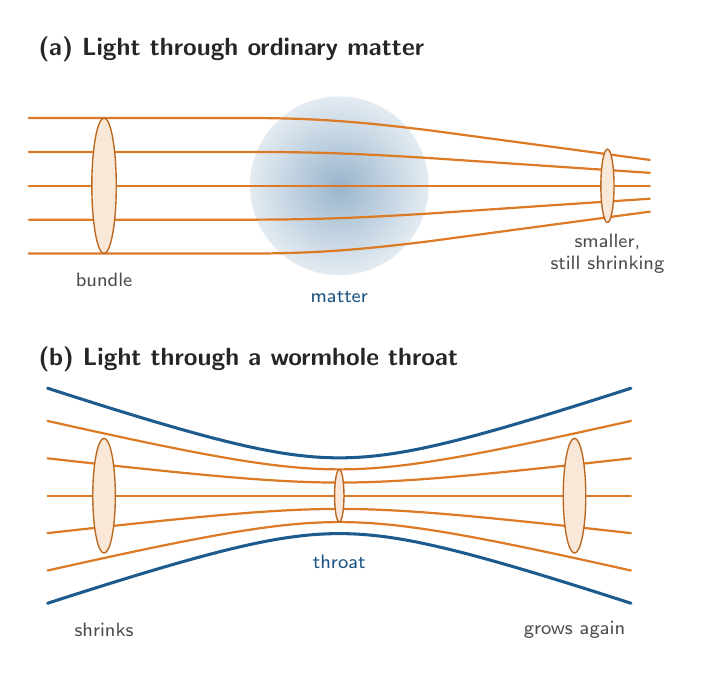
\begin{tikzpicture}[x=34pt, y=34pt,
  ray/.style={seorange, line width=0.8pt},
  section/.style={draw=seorange!85!black, fill=seorange!18, line width=0.5pt},
  ttl/.style={font=\sffamily\bfseries\small, text=black!85, anchor=west},
  note/.style={font=\sffamily\scriptsize, text=black!70},
]
% ------------------------------------------------------------- (a)
\begin{scope}[yshift=112pt]
\node[ttl] at (-3.3,1.45) {(a) Light through ordinary matter};
\shade[inner color=seblue!45, outer color=seblue!12] (0,0) circle (0.95);
\node[note, text=seblue!90!black] at (0,-1.18) {matter};
\foreach \y in {-0.72,-0.36,0,0.36,0.72} {
  \draw[ray] (-3.3,\y) -- (-0.95,\y)
    .. controls (-0.2,\y) and (0.3,{0.93*\y}) .. (0.95,{0.82*\y})
    -- (3.3,{0.82*\y - (3.3-0.95)*0.82*\y/4.4});
}
\draw[section] (-2.5,0) ellipse (0.13 and 0.72);
\draw[section] (2.85,0) ellipse (0.07 and 0.39);
\node[note] at (-2.5,-1.0) {bundle};
\node[note, align=center] at (2.85,-0.72) {smaller,\\still shrinking};
\end{scope}

% ------------------------------------------------------------- (b)
\begin{scope}
\node[ttl] at (-3.3,1.45) {(b) Light through a wormhole throat};
\foreach \s in {1,-1}
  \draw[seblue, line width=1.1pt, domain=-3.1:3.1, samples=80, variable=\x]
    plot (\x, {\s*sqrt(0.35^2 + (0.3*\x)^2)*1.15});
\foreach \f in {-0.8,-0.4,0,0.4,0.8}
  \draw[ray, domain=-3.1:3.1, samples=80, variable=\x]
    plot (\x, {\f*sqrt(0.35^2 + (0.3*\x)^2)});
\draw[section] (-2.5,0) ellipse (0.12 and 0.61);
\draw[section] (0,0) ellipse (0.05 and 0.28);
\draw[section] (2.5,0) ellipse (0.12 and 0.61);
\node[note] at (-2.5,-1.42) {shrinks};
\node[note, text=seblue!90!black] at (0,-0.7) {throat};
\node[note] at (2.5,-1.42) {grows again};
\end{scope}
\end{tikzpicture}
\end{document}
